%source mathadata
\begin{minipage}{0.42\textwidth}

		Un algorithme cherche la droite qui sépare au mieux les points blancs et les points noirs en minimisant le nombre d'erreurs.

		\begin{itemize}
			\item L'algorithme utilise des droites parallèles à une droite de référence $D_1$.
			\item Pour une droite donnée, un point au-dessus est considéré noir, un point en dessous est considéré blanc.
			\item Pour chaque droite, l'algorithme calcule le pourcentage d'erreur.
			\item L'algorithme sélectionne la droite qui minimise ce pourcentage.
		\end{itemize}

	\end{minipage}
	\hfill
	\begin{minipage}{0.55\textwidth}
		\begin{center}
			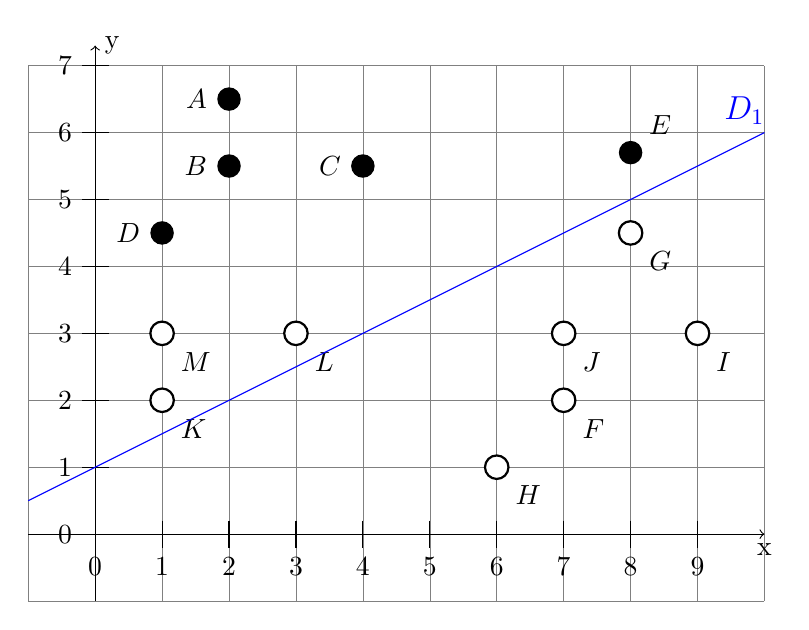
\begin{tikzpicture}[scale=0.85]
				% \tikzstyle{subj} = [circle, minimum width=4pt, fill, inner sep=0pt]
				% \tikzstyle{obj}  = [circle, minimum width=8pt, draw, inner sep=0pt]

				\tikzset{
					grid major/.style = {very thin, gray},
					grid minor/.style = {very thin, lightgray}
				}
				\draw[grid major] (-1, -1) grid[step=1] (10, 7);
				\draw[->] (-1,0) -- (10,0) node[below] {x};
				\draw[->] (0,-1) -- (0,7.3) node[right] {y};
				\foreach \x in {0,1,...,9} \draw (\x,0.2) -- (\x,-0.2) node[below] {\x};
				\foreach \y in {0,1,...,7} \draw (0.2,\y) -- (-0.2,\y) node[left] {\y};
				\node at (2,6.5) [circle,fill,inner sep=3pt,label=left:{$A$}] {}; % Mouton A
				\node at (2,5.5) [circle,fill,inner sep=3pt,label=left:{$B$}] {}; % Mouton B
				\node at (4,5.5) [circle,fill,inner sep=3pt,label=left:{$C$}] {}; % Mouton C
				\node at (1,4.5) [circle,fill,inner sep=3pt,label=left:{$D$}] {}; % Mouton D
				\node at (8,5.7) [circle,fill,inner sep=3pt,label=above right:{$E$}] {}; % Mouton E
				\node at (7,2) [circle,fill=white,thick,draw,inner sep=3pt,label=below right:{$F$}] {}; % Vache F
				\node at (8,4.5) [circle,fill=white,thick,draw,inner sep=3pt,label=below right:{$G$}] {}; % Vache G
				\node at (6,1) [circle,fill=white,thick,draw,inner sep=3pt,label=below right:{$H$}] {}; % Vache H
				\node at (9,3) [circle,fill=white,thick,draw,inner sep=3pt,label=below right:{$I$}] {}; % Vache I
				\node at (7,3) [circle,fill=white,thick,draw,inner sep=3pt,label=below right:{$J$}] {}; % Vache J
				\node at (1,2) [circle,fill=white,thick,draw,inner sep=3pt,label=below right:{$K$}] {}; % Vache K
				\node at (3,3) [circle,fill=white,thick,draw,inner sep=3pt,label=below right:{$L$}] {}; % Vache L
				\node at (1,3) [circle,fill=white,thick,draw,inner sep=3pt,label=below right:{$M$}] {}; % Vache M
				\draw[ domain=-1:10, smooth, variable=\x, blue]   plot ({\x}, {0.5*\x+1});
				\node[above=3pt, font=\large\bfseries, blue] at ({9.7}, {0.5*9.7+1}) {$D_1$};
				%\draw[ domain=0:9, smooth, variable=\x, green] plot ({\x}, {0.5*\x+2});
				%\draw[ domain=0:9, smooth, variable=\x, green] plot ({\x}, {0.5*\x+3});
				% \draw[ domain=0:9, smooth, variable=\x, green] plot ({\x}, {0.3*\x+3});
				%\draw[ domain=0:9, smooth, variable=\x, green] plot ({\x}, {0.5*\x});
			\end{tikzpicture}
		\end{center}
	\end{minipage}

	\vspace{0.3cm}

	\begin{multicols}{2}

		\begin{MADenumerate}
			\item Quelle est l'équation de la droite $D_1$ ?

			\item Calcul du pourcentage d'erreur associé à cette droite.
			\begin{enumerate}
				\item Compter le nombre de points du mauvais côté de la droite.
				\item Déduire le pourcentage d'erreur associé à cette droite.

			\end{enumerate}
			\item L'algorithme améliore le pourcentage d'erreur en traçant d'autres droites parallèles à $D_1$. Pour cela, on modifie pas à pas $p$ en gardant le même $m$.
			\begin{enumerate}
				\item Tracez la droite $D_2$ d'équation \\$y=0{,}5x+2$.
				\item Calculer le nouveau pourcentage d'erreur.
				\item Continuer de même en traçant plusieurs droites $D_3$, $D_4$ et $D_5$ parallèles à $D_1$ et $D_2$ sans oublier de donner leurs équations et de calculer le pourcentage d'erreur à chaque fois.

			\end{enumerate}
			\item Avec cette méthode, quelle est la droite qui fait le moins d'erreurs ?
			\item Avec la droite de la question précédente, le point $W(2;3{,}5)$ est-il considéré comme un point blanc ou comme un point noir ?

			\item Bonus : Il est possible
			de réduire encore le pourcentage d'erreur.
			\begin{enumerate}
				\item Trouver une droite permettant de réduire encore le pourcentage d'erreur. (Vous pouvez changer le coefficient directeur $m$ cette fois-ci.)
				\item Déterminer l'équation de cette droite.
			\end{enumerate}

		\end{MADenumerate}

	\end{multicols}
